%\begin{center}
%\begin{minipage}{.5\textwidth}
\begin{tikzpicture}[scale=0.33] %[x={10.0pt},y={10.0pt}] 
    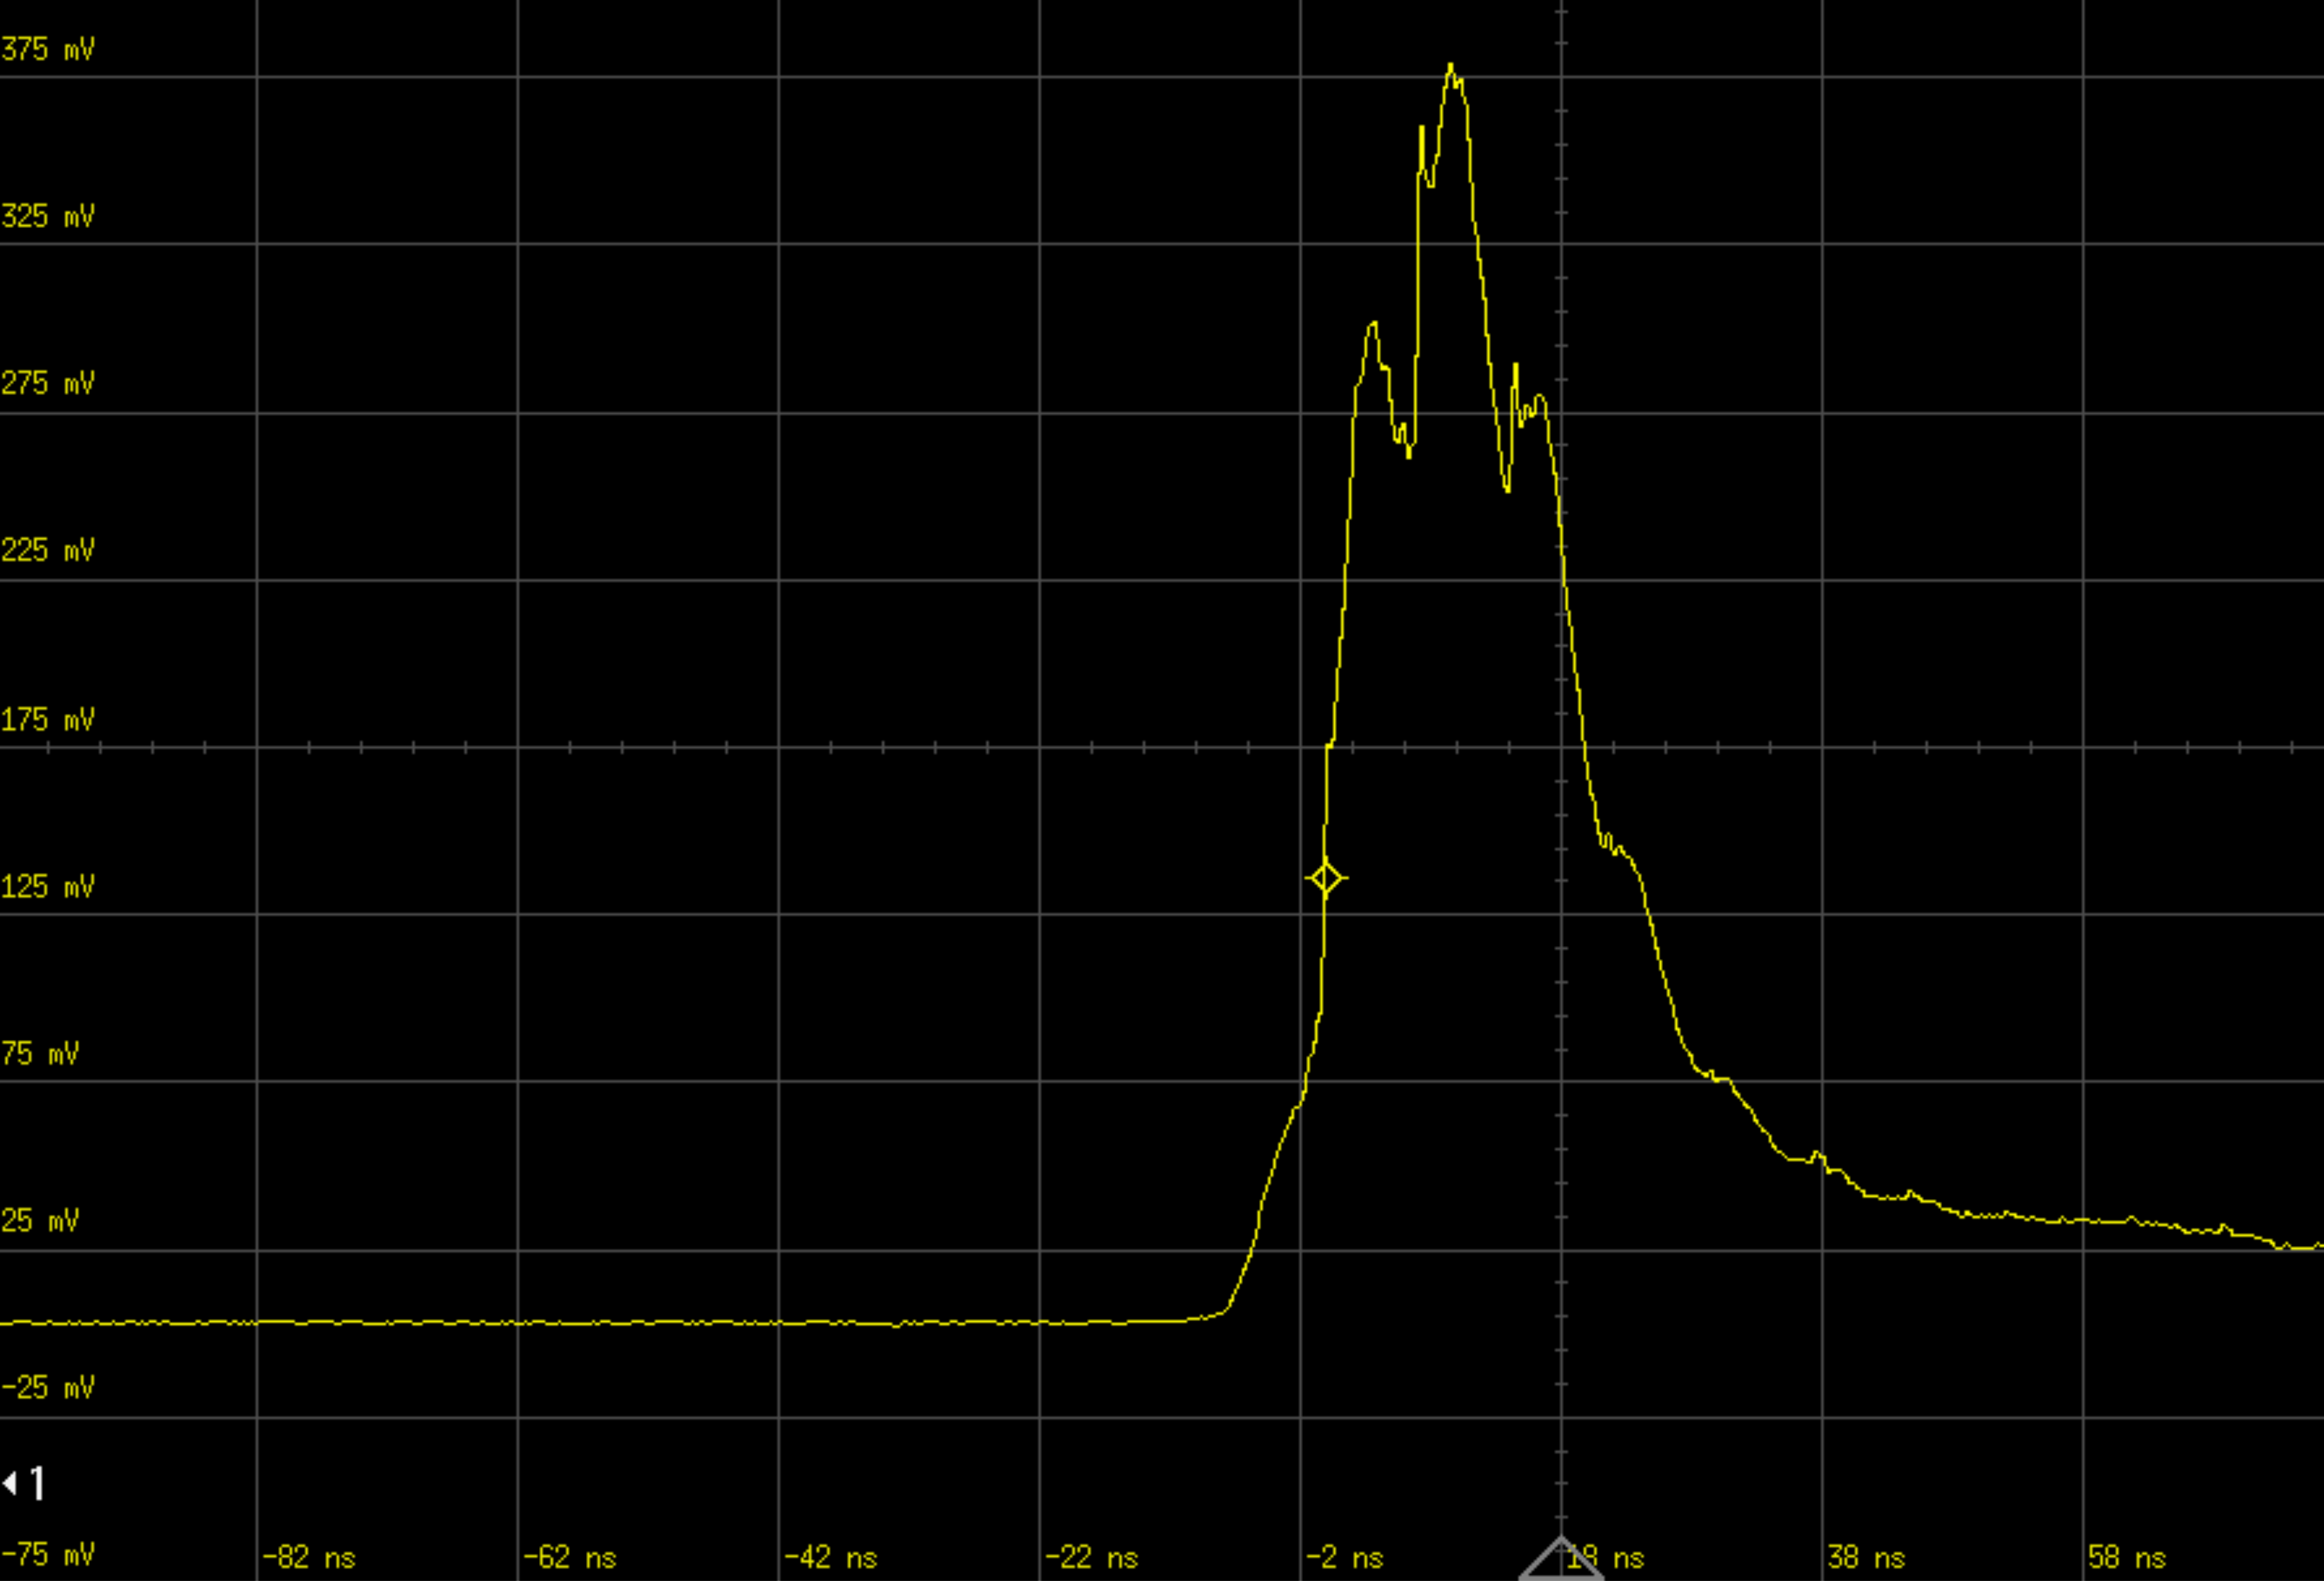
\includegraphics[width=0.4\textwidth,valign=c]{img/Temporal profile Litron Corel.png} 
\end{tikzpicture}% NO EMPTY LINE HERE!!!!
%\end{minipage}
%\begin{minipage}{.5\textwidth}
\qquad % <----------------- SPACE BETWEEN PICTURES
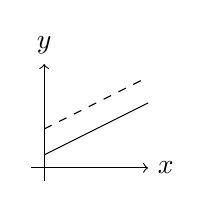
\begin{tikzpicture}[scale=0.33] %[x={10.0pt},y={10.0pt}]
      \draw[->] (-0.5,0) -- (4,0) node[right] {$x$};  
      \draw[->] (0,-0.5) -- (0,4) node[above] {$y$};  
      \draw (0,0.5) -- (4,2.5);  
      \draw [dashed] (0,1.5) -- (4,3.5);  
\end{tikzpicture} 
%\end{minipage}
\caption{Left: No Interaction. Right: Interaction} \label{fig:M} 
%\end{center}


    \section*{Residual stress measurement}
    The residual stress measurements were carried out using the incremental centre hole-drilling (ICHD) technique and X-ray diffraction using conventional X-ray diffraction \(\sin ^2(\Psi )\) technique. The hole drilling system PRISM by Stresstech company was used to gain depth-resolved residual stress profiles. A Rigaku XRD Automate 2 instrument and electrolytic removal was used for analyzing residual stresses in two orthogonal directions. XRD residual stress measurement parameters are provided in Table. 

        %%%%%%%%%%%%%%%%%%%%%%%%%%%%%%%%%%%%%%%%%%%%%%%%%%%%%%%%%%%%%%%%%
    %%%%%%%%%%%%%%%%%%%%%%%%%%%%%%%%%%%%%%%%%%%%%%%%%%%%%%%%%%%%%%%%%
    %%%%%%%%%%%%%%%%%%%%%%%%%%%%%%%%%%%%%%%%%%%%%%%%%%%%%%%%%%%%%%%%%
    % XRD parameters
    \begin{center}  

    \begin{threeparttable}
        \centering
        \begin{tabular}{|c | c|} 
        \hline
            \textbf{Item} & \textbf{Description} \\ [0.5ex] 
        \hline
        Detector & PSSD(Position sensitive scintillation detector)  \\ 
        \hline
            Radiation & MnK\(\alpha_1\)(\lambda = 2.1 )  \\
        \hline
            Tilt Angles [\degree] & \textless 0.5  \\ 
        \hline
            Aperture size(diameter) [mm] & 1 \\
        \hline
            Plane(Bragg's Angle) [\degree]  & \{311\} set of planes.Bragg's angle:152\degree \\

        \hline
        \end{tabular}

        \caption[Litron~LPY~ST~7875-10~2HG parameters]{Parameters for XRD residual stress measurement}
        
       
    \end{threeparttable}

    \label{tab:xrdparameters}
    \end{center}